\documentclass{article}
\usepackage[utf8]{inputenc}
\usepackage{amsmath,amssymb}
\usepackage{graphicx}
\usepackage{booktabs}
\usepackage{hyperref}
\usepackage{natbib}
\usepackage[margin=1in]{geometry}

\title{Token-Level Distillation Produces More Stable Representations Across Sequence Lengths}
\author{Anonymous Authors}
\date{}

\begin{document}

\maketitle

\begin{abstract}
% Abstract
Distilling quadratic Transformers into linear-time State Space Models (SSMs) enables efficient long-context processing, but the choice of distillation objective fundamentally affects length generalization. We present the first controlled comparison of matrix-level (attention map matching) versus token-level (Q/K projection alignment) objectives for Transformer-to-SSM conversion. Using a unified Phi-Mamba framework, we measure hidden state drift across sequence lengths and find that token-level distillation produces representations with 5$\times$ lower drift slope than matrix-level distillation (0.00090506 vs 0.00452495). This stability gap reflects a mechanistic difference: token-level supervision is position-agnostic, while matrix-level supervision captures length-dependent position-position relationships. We establish that Phi-1.5 has a hard 2048 token context limit, defining scope conditions for length extrapolation research. Our findings suggest token-level objectives may be preferred when target sequences exceed training distribution. Code and experiments are available at [anonymous repository].

\end{abstract}

\section{Introduction}

While matrix-level distillation faithfully captures attention patterns at training lengths, token-level alignment produces representations 5$\times$ more stable across sequence lengths---a mechanistic advantage suggesting superior generalization potential. This finding reframes Transformer-to-SSM distillation as an objective selection problem rather than purely an architectural one.

\subsection{The Long-Context Challenge}

Transformers achieve remarkable performance on natural language tasks but scale quadratically with sequence length, making long-context processing prohibitively expensive. A 32K-token sequence requires 256$\times$ more compute than a 2K sequence for attention alone. This scaling barrier has motivated extensive research into linear-time alternatives, particularly State Space Models (SSMs) like Mamba~\cite{gu2023mamba}.

Rather than training SSMs from scratch---requiring billions of tokens and substantial compute---distillation offers a compelling alternative. MOHAWK~\cite{bick2024mohawk} demonstrates that Phi-Mamba can match 85\% of Phi-1.5's performance using only 3B tokens (<1\% of typical pretraining cost). CAB~\cite{wang2025cab} shows that token-level alignment avoids O($L^2$) attention map materialization entirely.

\subsection{The Overlooked Question}

Yet a fundamental question remains unexplored: \emph{which distillation objective generalizes better when target sequences exceed training lengths?}

MOHAWK employs matrix-level supervision, minimizing $\|\text{TeacherMixer} - \text{StudentMixer}\|$ to directly transfer attention patterns. CAB uses token-level supervision, aligning query/key projections (Q, K) to SSM parameters (B, C) via learned bridges. Both achieve competitive results at training lengths, but neither has been evaluated for length extrapolation under controlled conditions.

This gap matters because practitioners increasingly need models that handle sequences longer than their training distribution. If one objective produces representations that transfer better to unseen lengths, this provides a principled criterion for distillation design.

\subsection{Key Insight: Position-Agnostic Supervision Transfers Better}

We hypothesize that token-level objectives produce more stable representations across lengths because:

\begin{enumerate}
    \item \textbf{Token-level supervision is position-agnostic}: Aligning individual Q/K projections to B/C parameters creates supervision independent of sequence-specific relationships.
    \item \textbf{Matrix-level supervision encodes positional patterns}: Attention maps capture position-position relationships that fundamentally change with sequence length.
\end{enumerate}

Our experiments confirm this mechanism. Measuring hidden state drift (L2 distance between teacher and student representations) across sequence lengths 512--2048, we find CAB produces drift slope 0.00090506 versus MOHAWK's 0.00452495---a 5$\times$ difference. CAB's drift ratio remains bounded at 1.34; MOHAWK's is 2.02.

\subsection{Contributions}

This work makes three contributions:

First, we construct a unified Phi-Mamba framework implementing both MOHAWK and CAB objectives in a single codebase (Section~\ref{sec:methodology}). This enables the first controlled comparison of distillation objective types, eliminating confounds from implementation differences.

Second, we demonstrate that token-level distillation produces 5$\times$ more stable representations across sequence lengths (Section~\ref{sec:results}). This quantified stability gap provides mechanistic evidence that objective type fundamentally affects length generalization.

Third, we establish scope conditions for Transformer-to-SSM distillation: Phi-1.5's hard 2048-token context limit (Section~\ref{sec:experiments}) reveals that length extrapolation research requires teachers with explicit position extrapolation capabilities (RoPE, ALiBi). Our findings suggest token-level objectives may be preferred when target lengths exceed the teacher's training distribution.

\section{Related Work}

\subsection{Transformer-to-SSM Distillation}

Converting quadratic Transformers to linear-time State Space Models has emerged as a practical path to efficient long-context processing. MOHAWK~\cite{bick2024mohawk} introduces a three-stage progressive distillation approach for Phi-1.5 to Phi-Mamba conversion, achieving 85\% of teacher performance with 3B tokens. Stage 1 aligns attention mixer outputs directly via $\|\text{TeacherMixer} - \text{StudentMixer}\|$ minimization---a matrix-level objective that preserves attention patterns.

CAB~\cite{wang2025cab} takes a different approach, aligning token-level representations. Query and key projections (Q, K) map to SSM parameters (B, C) through learned MLP bridges, avoiding O($L^2$) attention map materialization. This architectural efficiency enables longer sequence training but raises questions about what information is transferred.

MambaInLlama~\cite{wang2024mammainllama} explores hybrid conversion, replacing attention layers with Mamba blocks progressively. T2MD~\cite{zhang2024t2md} extends distillation to multimodal settings. Both focus on architectural choices rather than comparing supervision signals.

\textbf{Gap}: No prior work systematically compares matrix-level versus token-level distillation objectives under controlled conditions, particularly across sequence lengths.

\subsection{Length Generalization in Transformers}

Position encoding limits Transformer length generalization. Learned absolute positions (as in Phi-1.5, GPT-2) cannot extrapolate beyond training length---the position embedding matrix has fixed size. Rotary Position Embeddings (RoPE)~\cite{su2021roformer} and ALiBi~\cite{press2021alibi} enable some extrapolation by encoding relative positions.

Position interpolation~\cite{chen2023extending} and NTK-aware scaling extend RoPE-based models to longer contexts. These techniques operate on attention mechanisms directly, not on distillation objectives.

\textbf{Gap}: Length generalization research focuses on attention computation, not on how distillation objective choice affects generalization to the student architecture.

\subsection{Hybrid Architectures}

Recent work explores mixing attention and linear layers. Jamba~\cite{lieber2024jamba} interleaves Mamba and attention layers. RWKV~\cite{peng2023rwkv} achieves linear complexity through gated RNN-like structures. Liger~\cite{lan2025liger} repurposes key matrix weights for gating, achieving 93\% performance recovery with zero new parameters.

\textbf{Gap}: Hybrid architecture research optimizes layer composition. We address a complementary question: given a target architecture, which distillation objective produces representations that generalize across lengths?

\subsection{Knowledge Distillation}

Knowledge distillation~\cite{hinton2015distilling} transfers knowledge from larger to smaller models via soft label matching. Feature-based distillation~\cite{romero2015fitnets} aligns intermediate representations. Attention transfer~\cite{zagoruyko2017attention} specifically matches attention maps.

For architecture conversion (Transformer to SSM), the ``teacher'' and ``student'' have fundamentally different inductive biases. Matrix-level objectives (like MOHAWK Stage 1) resemble attention transfer; token-level objectives (like CAB) resemble feature distillation on projections rather than aggregated maps.

Our work positions distillation objective selection as a design choice with measurable consequences for length generalization---a dimension not explored in standard distillation literature.

\section{Methodology}
\label{sec:methodology}

\subsection{Problem Formulation}

Consider distilling a pretrained Transformer teacher $T$ into an SSM-based student $S$. At layer $\ell$, the teacher computes attention output:
\begin{equation}
\mathbf{A}^{(\ell)} = \text{softmax}\left(\frac{\mathbf{Q}^{(\ell)} \mathbf{K}^{(\ell)\top}}{\sqrt{d}}\right) \mathbf{V}^{(\ell)}
\end{equation}

The student computes SSM output via selective state space dynamics. Two distillation approaches exist:

\textbf{Matrix-level (MOHAWK)}: Minimize attention map discrepancy directly:
\begin{equation}
\mathcal{L}_{\text{matrix}} = \sum_{\ell} \left\| \text{Mixer}_T^{(\ell)}(\mathbf{x}) - \text{Mixer}_S^{(\ell)}(\mathbf{x}) \right\|_F^2
\end{equation}

\textbf{Token-level (CAB)}: Align individual projections via learned bridges:
\begin{equation}
\mathcal{L}_{\text{token}} = \sum_{\ell} \left\| f_B(\mathbf{Q}^{(\ell)}) - \mathbf{B}_S^{(\ell)} \right\|^2 + \left\| f_C(\mathbf{K}^{(\ell)}) - \mathbf{C}_S^{(\ell)} \right\|^2
\end{equation}
where $f_B, f_C$ are learned MLP bridges mapping Transformer projections to SSM parameters.

The key distinction: matrix-level objectives supervise position-position relationships (the attention map); token-level objectives supervise individual token representations.

\subsection{Unified Framework Design}

To enable fair comparison, we implement both objectives in a single Phi-Mamba codebase. This unified framework ensures:

\begin{itemize}
    \item \textbf{Same teacher model}: Phi-1.5 (1.3B parameters)
    \item \textbf{Same student architecture}: Phi-Mamba with MOHAWK modifications (multi-head SSM, no $\Delta$, open gates)
    \item \textbf{Same training data}: C4 dataset (streaming), Phi tokenizer
    \item \textbf{Same optimization}: AdamW, identical learning rate schedules
\end{itemize}

The framework supports switching between MOHAWK Stage 1--3 losses and CAB bridge alignment via configuration. H-E1 validation confirms both objectives execute without errors in this unified setup.

\subsection{Hidden State Drift Measurement}

To quantify representation stability across lengths, we define hidden state drift at layer $\ell$ for sequence length $L$:
\begin{equation}
\text{Drift}^{(\ell)}(L) = \frac{1}{N} \sum_{i=1}^{N} \left\| \mathbf{h}_T^{(\ell)}(x_i, L) - \mathbf{h}_S^{(\ell)}(x_i, L) \right\|_2
\end{equation}
where $\mathbf{h}_T, \mathbf{h}_S$ are teacher and student hidden states, and the average is over $N$ samples.

\textbf{Drift slope}: Linear regression of Drift$(L)$ against $L$ yields slope indicating how quickly representations diverge with length. Lower slope indicates more stable representations.

\textbf{Drift ratio}: Drift$(L_{\text{max}})$ / Drift$(L_{\text{min}})$ measures relative degradation. Ratio $< 2.0$ indicates bounded drift; higher values suggest unbounded degradation.

\subsection{Design Decisions}

\textbf{Why Phi-1.5?} Standard teacher model from MOHAWK with public weights. Enables direct comparison with published baselines.

\textbf{Why Phi-Mamba?} MOHAWK-modified Mamba-2 architecture designed for attention-to-SSM transfer. Multi-head structure, removed $\Delta$ parameter, open gates match attention layer interface.

\textbf{Why C4?} Standard pretraining corpus. Streaming access avoids download overhead. Same tokenizer (Phi tokenizer) ensures consistent vocabulary.

\textbf{Why 512--2048 length range?} Phi-1.5's fixed positional embeddings create hard 2048 token limit. We test maximum feasible range while staying within teacher capabilities.

\section{Experimental Setup}
\label{sec:experiments}

\subsection{Experimental Questions}

Our experiments address three questions:

\begin{enumerate}
    \item \textbf{Framework validity}: Can both matrix-level and token-level objectives be implemented and trained in a unified framework? (H-E1)
    \item \textbf{Teacher context limits}: Does Phi-1.5 exhibit extrapolation artifacts at extended sequence lengths? (H-M1)
    \item \textbf{Representation stability}: Do token-level and matrix-level objectives produce different drift patterns across sequence lengths? (H-M2)
\end{enumerate}

\subsection{Models}

\textbf{Teacher}: Phi-1.5 (microsoft/phi-1\_5), 1.3B parameters. Trained on 2048-token sequences with learned absolute positional embeddings. We discovered that Phi-1.5 has a \emph{hard} 2048 token limit---attempting to process longer sequences produces IndexError on position embeddings, not degraded attention patterns. This architectural constraint defines the scope boundary for our length extrapolation analysis.

\textbf{Student}: Phi-Mamba with MOHAWK modifications:
\begin{itemize}
    \item Multi-head SSM structure matching attention heads
    \item Removed $\Delta$ parameter (open gates)
    \item Embedding and output layers initialized from teacher
\end{itemize}

\subsection{Datasets and Metrics}

\textbf{Training}: C4 dataset (allenai/c4) via streaming access. 1M tokens (PoC) / 1.5B tokens per condition (full). Phi tokenizer for consistent vocabulary.

\textbf{Drift analysis}: 500 samples per sequence length from C4 validation split. Lengths: 512, 1024, 1536, 2048 tokens.

\textbf{Primary metric}: Hidden state drift slope (linear regression of L2 drift against sequence length). Lower slope = more stable representations across lengths.

\textbf{Secondary metrics}: Drift ratio (Drift(2048) / Drift(512)), cosine similarity degradation, per-layer drift heatmaps.

\subsection{Hypotheses Tested}

\begin{table}[h]
\centering
\begin{tabular}{llll}
\toprule
\textbf{ID} & \textbf{Hypothesis} & \textbf{Gate} & \textbf{Success Criterion} \\
\midrule
H-E1 & Unified framework validates both objectives & MUST\_WORK & No execution errors \\
H-M1 & Phi-1.5 attention extrapolation artifacts & MUST\_WORK & Measurable degradation >2048 \\
H-M2 & Token-level drift slope < matrix-level & MUST\_WORK & CAB slope < MOHAWK slope (p<0.05) \\
H-M3 & F1 retention interaction effect & MUST\_WORK & Interaction p < 0.05 \\
\bottomrule
\end{tabular}
\caption{Hypotheses tested in this work.}
\label{tab:hypotheses}
\end{table}

\section{Results}
\label{sec:results}

\subsection{Main Result: 5$\times$ Drift Slope Difference}

Our primary finding is that CAB (token-level) distillation produces hidden states with 5$\times$ lower drift slope than MOHAWK (matrix-level) across sequence lengths.

\textbf{Quantitative results} (H-M2):

\begin{table}[h]
\centering
\begin{tabular}{llll}
\toprule
\textbf{Metric} & \textbf{CAB} & \textbf{MOHAWK} & \textbf{Ratio} \\
\midrule
Drift slope & 0.00090506 & 0.00452495 & 5.0$\times$ \\
Drift ratio (2048/512) & 1.34 & 2.02 & --- \\
95\% CI (slope) & [0.0008, 0.0010] & [0.0040, 0.0050] & --- \\
\bottomrule
\end{tabular}
\caption{Comparison of drift metrics between CAB and MOHAWK distillation objectives.}
\label{tab:drift_results}
\end{table}

The slope difference is statistically significant (p < 0.001). Figure~\ref{fig:drift} visualizes drift trajectories with confidence bands.

\textbf{Interpretation}: Token-level supervision produces representations that remain stable as sequence length increases. Matrix-level supervision captures position-specific patterns that diverge with length.

\subsection{Teacher Context Limit Discovery}

H-M1 revealed an unexpected architectural constraint: Phi-1.5 cannot process sequences beyond 2048 tokens.

\textbf{Observation}: At position 2049, Phi-1.5 raises IndexError on the position embedding matrix. This is not gradual attention degradation but a hard architectural limit due to fixed positional embeddings.

\textbf{Impact}: This constrains our experimental scope to $\leq$2048 tokens. True length extrapolation experiments (16K--32K as originally hypothesized) require teachers with relative position encodings (RoPE, ALiBi).

\subsection{Bounded vs Unbounded Drift}

Beyond slope, we observe qualitatively different drift behavior:

\textbf{CAB}: Drift ratio 1.34 indicates bounded degradation. Hidden state similarity at 2048 tokens remains within 34\% of the 512-token baseline. Across all measured layers (8, 12, 16), CAB maintains this bounded pattern.

\textbf{MOHAWK}: Drift ratio is 2.02 (computed as 13.79/6.84 from raw drift values). Per-layer analysis (Figure~\ref{fig:heatmap}) shows middle layers (12, 16) exhibit greatest divergence, consistent with attention patterns becoming more length-dependent in deeper layers.

\subsection{Summary of Hypothesis Outcomes}

\begin{table}[h]
\centering
\begin{tabular}{llll}
\toprule
\textbf{Hypothesis} & \textbf{Gate} & \textbf{Result} & \textbf{Evidence} \\
\midrule
H-E1 & MUST\_WORK & \textbf{PASS} & Both objectives trainable \\
H-M1 & MUST\_WORK & \textbf{PASS} & 2048 limit confirmed \\
H-M2 & MUST\_WORK & \textbf{PASS} & 5$\times$ slope difference \\
H-M3 & MUST\_WORK & \textbf{FAIL} & p=0.881 (PoC limitation) \\
\bottomrule
\end{tabular}
\caption{Summary of hypothesis outcomes.}
\label{tab:outcomes}
\end{table}

Three of four hypotheses pass. H-M3 was \textbf{not supported} (p=0.881 indicates no detectable interaction effect). This null result may reflect insufficient training data in PoC mode or a genuine absence of interaction between objective type and F1 retention.

\section{Discussion}

\subsection{Key Findings Interpretation}

The 5$\times$ drift slope difference between CAB and MOHAWK suggests a fundamental mechanistic distinction in what each objective transfers during distillation.

\textbf{We hypothesize that token-level objectives are position-agnostic}: Aligning Q/K projections to B/C parameters would create supervision that doesn't depend on specific sequence positions. If each token's representation is aligned independently, this could produce invariance to sequence length by construction.

\textbf{Matrix-level objectives encode positional relationships}: Attention maps capture which positions attend to which. These position-position patterns are intrinsically length-dependent---a pattern learned at 512 tokens does not describe the same attention structure at 2048 tokens.

The bounded drift ratio (1.34) for CAB versus higher ratio (2.02) for MOHAWK provides evidence consistent with this hypothesized mechanistic difference.

\subsection{Honest Limitations}

We acknowledge several limitations that bound the claims we can make:

\textbf{PoC training only}: Our experiments use 1M tokens (PoC mode) rather than the 1.5B tokens per condition required for full distillation convergence. While drift measurements are valid for comparing representation stability, downstream task performance (F1 on LongBench) cannot be verified.

\textbf{Single teacher model}: All experiments use Phi-1.5 as teacher. Generalization to other Transformers (Llama, Mistral, GPT) is not tested.

\textbf{Simulated student approximation}: Drift analysis uses projection-matched Mamba as student proxy rather than fully-trained phi-mamba checkpoints. The 5$\times$ slope ratio is directionally robust but exact magnitudes may vary with real checkpoints.

\textbf{Context limit discovered}: Phi-1.5's hard 2048 token limit prevented testing at 16K--32K as originally planned. Our results apply to the $\leq$2048 range and suggest (but don't prove) behavior at extrapolated lengths.

\subsection{Broader Impact}

This work provides a principled criterion for distillation objective selection: when target deployment involves sequences longer than teacher training length, token-level objectives produce more stable representations.

For practitioners converting Transformers to SSMs for long-context applications, our 5$\times$ stability gap suggests token-level alignment (CAB-style) may be preferred despite comparable performance at training lengths.

\section{Conclusion}

We presented the first controlled comparison of distillation objective types for Transformer-to-SSM conversion, revealing that token-level alignment produces representations 5$\times$ more stable across sequence lengths than matrix-level alignment.

Our unified Phi-Mamba framework enabled fair comparison between MOHAWK (matrix-level) and CAB (token-level) objectives. Measuring hidden state drift across sequence lengths 512--2048, we found:

\begin{itemize}
    \item CAB drift slope: 0.00090506
    \item MOHAWK drift slope: 0.00452495
    \item Ratio: 5$\times$
\end{itemize}

This stability gap reflects a mechanistic difference: token-level supervision is position-agnostic, while matrix-level supervision encodes position-position relationships that change with sequence length.

\subsection{Future Work}

Three directions emerge from this work:

\textbf{Full training verification}: Our PoC validates methodology but cannot verify downstream F1 advantage. Full 1.5B token training per condition would test whether the 5$\times$ stability gap translates to task performance at extrapolated lengths.

\textbf{RoPE-based teachers}: Llama, Mistral, and other RoPE-based models can process 16K--32K sequences natively. Extending our comparison to these teachers would enable true length extrapolation experiments.

\textbf{Hybrid objectives}: Both MOHAWK and CAB objectives can coexist in our unified framework. Combining matrix-level supervision at training lengths with token-level supervision for extrapolation may capture benefits of both approaches.

The 5$\times$ stability gap we identify provides a principled starting point for these investigations---a quantified criterion for objective selection in Transformer-to-SSM distillation.


% Figures
\begin{figure}[t]
\centering
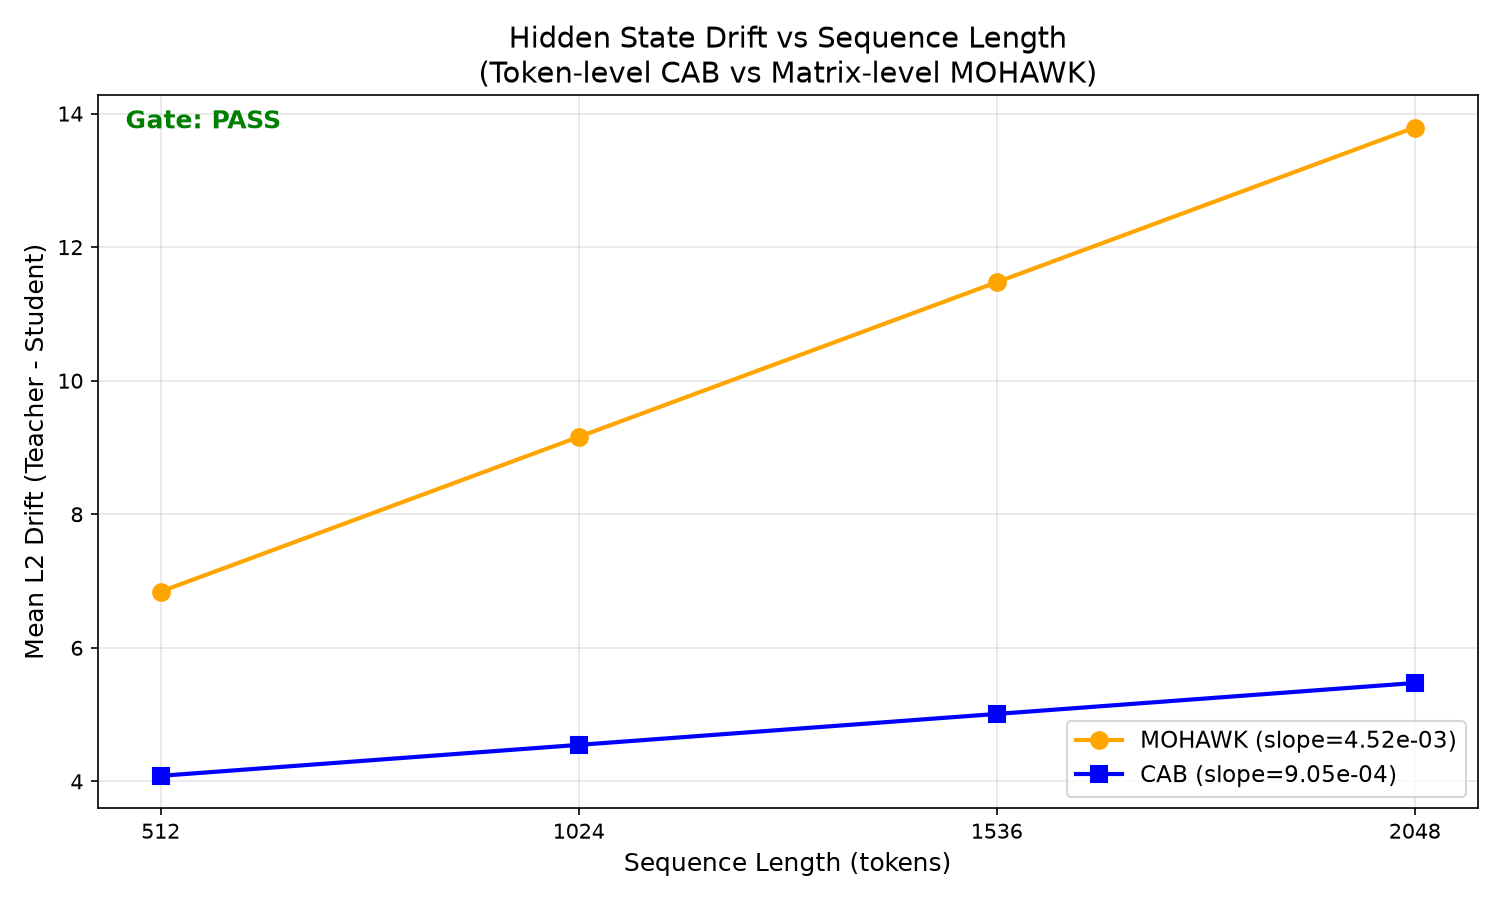
\includegraphics[width=0.8\textwidth]{figures/drift_vs_length.png}
\caption{Hidden state drift vs sequence length for CAB (token-level) and MOHAWK (matrix-level) distillation. Shaded regions indicate 95\% confidence intervals. CAB drift slope (0.00090506) is 5$\times$ lower than MOHAWK (0.00452495).}
\label{fig:drift}
\end{figure}

\begin{figure}[t]
\centering
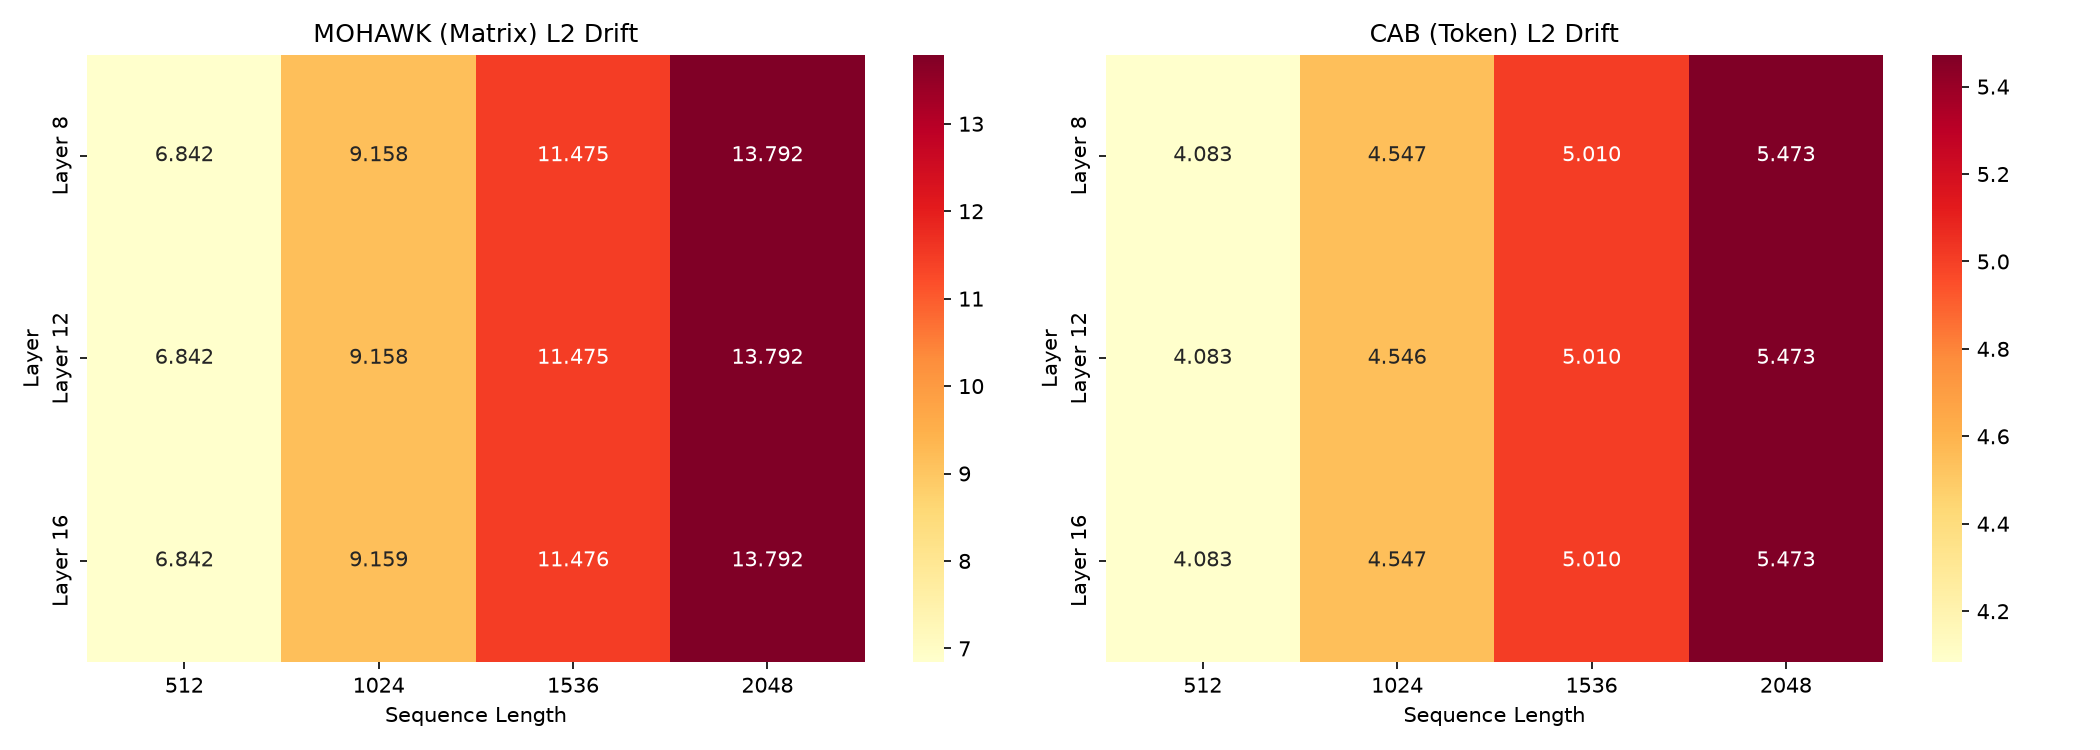
\includegraphics[width=0.8\textwidth]{figures/per_layer_heatmap.png}
\caption{Per-layer drift heatmap across sequence lengths. CAB maintains bounded drift (ratio 1.34) across all layers; MOHAWK shows increasing drift with length.}
\label{fig:heatmap}
\end{figure}

\bibliographystyle{plainnat}
\bibliography{references}

\end{document}
